% ---------- Titelblad Masterproef Faculteit Wetenschappen -----------
% Dit document is opgesteld voor compilatie met pdflatex.  Indien je
% wilt compileren met latex naar dvi/ps, dien je de figuren naar
% (e)ps-formaat om te zetten.
%                           -- december 2012
% -------------------------------------------------------------------
\RequirePackage{fix-cm}
\documentclass[12pt,a4paper,oneside]{book}

% --------------------- In te laden pakketten -----------------------
% Deze kan je eventueel toevoegen aan de pakketten die je al inlaadt
% als je dit titelblad integreert met de rest van thesis.
% -------------------------------------------------------------------
\usepackage{graphicx,xcolor,textpos}
\usepackage{helvet}
\usepackage[linktoc=all]{hyperref}
\usepackage[dutch]{babel}


% -------------------- Pagina-instellingen --------------------------
% Indien je deze wijzigt, zal het titelblad ook wijzigen.  Dit dien je
% dan manueel aan te passen.
% --------------------------------------------------------------------

\topmargin -10mm
\textwidth 160truemm
\textheight 240truemm
\oddsidemargin 0mm
\evensidemargin 0mm

% ------------------- textpos-instellingen ---------------------------
% Enkele andere instellingen voor het voorblad.
% --------------------------------------------------------------------

\definecolor{green}{RGB}{172,196,0}
\definecolor{bluetitle}{RGB}{29,141,176}
\definecolor{blueaff}{RGB}{0,0,128}
\definecolor{blueline}{RGB}{82,189,236}
\setlength{\TPHorizModule}{1mm}
\setlength{\TPVertModule}{1mm}

\begin{document}

% ---------------------- Voorblad ------------------------------------
% Vergeet niet de tekst aan te passen:
% - Titel en, indien van toepassing, ondertitel
%          voor eventuele formules in de titel of ondertitel
%          gebruik je  \form{$...$}
% - Je naam
% - Je (co)promotor, begeleider (indien van toepassing)
% - Je opleiding
% - Het academiejaar
% --------------------------------------------------------------------
\thispagestyle{empty}
\newcommand{\form}[1]{\scalebox{1.087}{\boldmath{#1}}}
\sffamily
%
\begin{textblock}{191}(-24,-11)
\colorbox{green}{\hspace{123mm}\ \parbox[c][18truemm]{68mm}{\textcolor{white}{FACULTEIT WETENSCHAPPEN}}}
\end{textblock}
%
\begin{textblock}{70}(-18,-19)
\textblockcolour{}
\includegraphics*[height=19.8truemm]{LogoKULeuven}
\end{textblock}
%
\begin{textblock}{160}(-6,63)
\textblockcolour{}
\vspace{-\parskip}
\flushleft
\fontsize{40}{42}\selectfont \textcolor{bluetitle}{Programmeren met Onzekerheid: een Case Study}\\[1.5mm]
%\fontsize{20}{22}\selectfont Ondertitel \form{$S=\pi r^2$\textsl{(facultatief)}}
\end{textblock}
%
\begin{textblock}{160}(8,153)
\textblockcolour{}
\vspace{-\parskip}
\flushright
\fontsize{14}{16}\selectfont \textbf{Sus VERWIMP}
\end{textblock}
%
\begin{textblock}{70}(-6,191)
\textblockcolour{}
\vspace{-\parskip}
\flushleft
Promotor: Prof. T. Schrijvers\\[-2pt]
\textcolor{blueaff}{Affiliatie \textsl{(facultatief)}}\\[5pt]
%Co-promotor: \textsl{(facultatief)}\\[-2pt]
%\textcolor{blueaff}{Affiliatie \textsl{(facultatief)}}\\[5pt]
Begeleider: \textsl{A. Vandenbroucke (facultatief)}\\[-2pt]
\textcolor{blueaff}{Affiliatie \textsl{(facultatief)}}\\
\end{textblock}
%
\begin{textblock}{160}(8,191)
\textblockcolour{}
\vspace{-\parskip}
\flushright
Proefschrift ingediend tot het\\[4.5pt]
behalen van de graad van\\[4.5pt]
Master of Science in\\[4.5pt]
Toegepaste Informatica\\
\end{textblock}
%
\begin{textblock}{160}(8,232)
\textblockcolour{}
\vspace{-\parskip}
\flushright
Academiejaar 2017-2018
\end{textblock}
%
\begin{textblock}{191}(-24,248)
{\color{blueline}\rule{550pt}{5.5pt}}
\end{textblock}
%
\vfill
\newpage

% Copyright statement
\textsf{\textcopyright} Copyright by KU Leuven
Zonder voorafgaande schriftelijke toestemming van zowel de promotor(en) als de auteur(s) is overnemen, kopiëren, gebruiken of realiseren van deze uitgave of gedeelten ervan verboden. Voor aanvragen tot of informatie i.v.m. het overnemen en/of gebruik en/of realisatie van gedeelten uit deze publicatie, wend u tot de KU Leuven, Faculteit Wetenschappen, Geel Huis, Kasteelpark Arenberg 11 bus 2100, 3001 Leuven (Heverlee), Telefoon +32 16 32 14 01.

Voorafgaande schriftelijke toestemming van de promotor(en) is eveneens vereist voor het aanwenden van de in dit afstudeerwerk beschreven (originele) methoden, producten, schakelingen en programma’s voor industrieel of commercieel nut en voor de inzending van deze publicatie ter deelname aan wetenschappelijke prijzen of wedstrijden.

\vfill
\newpage

% Als je het titelblad wil integreren met de rest van je thesis,
% kan je hieronder verder.
% ----------------------- Eerste pagina's -------------------------
% Hier kan je inhoudsopgave, voorwoord en dergelijke kwijt.
% -----------------------------------------------------------------
\rmfamily
\setcounter{page}{0}
\pagenumbering{roman}
\frontmatter
\chapter{Voorwoord}
\chapter{Korte Samenvatting}
\chapter{Lijst van afkortingen en lijst van symbolen}
\tableofcontents


\newpage
% ----------------------- Eigenlijke thesis -----------------------
% Vanaf de inleiding/het eerste hoofdstuk.
% -----------------------------------------------------------------
\mainmatter
\setcounter{page}{0}
\pagenumbering{arabic}
\chapter{Inleiding}
De grote interesse in het domein ‘onzekerheid’ in AI resulteerd in de ontwikkeling van verschillende programmeertalen. Deze talen worden probabilistische programmeertalen of PPL (Probabilistic Programming Language) genoemd. Een PPL heeft in grote lijnen 2 hoofdfuncties:
\begin{itemize}
	\item Het modelleren van een wereld met onzekerheid
	\item Het redeneren/infereren van vragen over deze wereld
\end{itemize}
Voorheen was het zeer moeilijk als programmeur om werelden met onzekerheid te modelleren, laat staan het redeneren over deze werelden. Met de komst van PPL’s is dit probleem al een stuk makkelijker geworden.
\\\\
Elke PPL heeft zijn eigen manier van implementatie en wordt vaak geimplementeerd als extensie op een general-purpose programmeertaal. Dit zorgt er voor dat de PPL niet gelimiteerd is aan een kleine subset van de werelden die het kan modelleren. Veel van deze PPL’s streven naar een balans tussen performantie en expressiviteit. Het is belangrijk voor een PPL om genoeg werelden te kunnen simuleren en op een aanneembare tijd te kunnen redeneren over vragen over deze wereld.
\\\\
Omdat er zo veel PPL’s beschikbaar zijn de laatste jaren is het niet altijd duidelijk welke voordelen of nadelen ze hebben ten opzichte van andere PPL’s. Verschillende van deze PPL’s zijn in recente artikels vergeleken met elkaar aan de hand van eigenschappen en concepten van de taal (Probabilistic (Logic) Programming Concepts, Luc De Raedt - Angelika Kimmig). Andere artikels vergelijken PPL’s aan de hand van hun vorige iteratie of PPL’s met hetzelfde programmeerparadigma (Inference and Learning in Probabilistic Logic Programs using Weighted Boolean Formulas, LUC DE RAEDT et al). 
\\\\
In deze thesis ga ben ik van plan PPL’s met een verschillend programmeerparadigma te evalueren. ik ga deze PPL’s evalueren ten opzichte van elkaar aan de hand van qualitatieve en quantitatieve criteria. Omdat het niet triviaal is om programmeertalen te vergelijken die totaal anders geimplementeerd zijn maak ik gebruik van een case study. Ik begin met het verzinnen van een onzekerheidsprobleem waarna ik uitleg geef waarom ik gekozen heb voor dit probleem. Daarna evalueer ik de implementatie van het probleem in de verschillende PPL’s aan de hand van vooropgestelde criteria. Ten slotte volgt een evaluatie van de PPL’s ten opzichte van elkaar. 
\\\\

Onzekerheid in artifici\"{e}le intelligentie is een van de invloedrijkste domeinen van artifici\"{e}le intelligentie. De reden hiervoor is omdat de wereld van nature veel onzekerheid bevat. Denk aan de volgende punten:
\begin{itemize}
	\item Kennis (we kunnen niet alles van de wereld weten)
	\item Incomplete modellen (verschijnselen die niet onder het model vallen)
	\item Sensoren (we kunnen de wereld enkel observeren met de tools die beschikbaar zijn en deze zijn meestal nog foutgevoelig.)
	\item Acties (we kunnen niet elke actie uitvoeren)
\end{itemize}
Als we spreken over werken met onzekerheid bedoelen we het opstellen van een hypothese, en deze hypothese (zo goed mogelijk) bewijzen aan de hand van het gegeven bewijs van de wereld.
Er zijn 3 belangrijke kwesties in verband met het werken met onzekerheid:
\begin{itemize}
	\item Representeren van onzekerheid
	\item Redeneren over onzekerheid
	\item Leren aan de hand van onzekerheid
\end{itemize}
Het representeren van onzekerheid gebeurd in het model. Een model is een weergave van een onzekerheidsprobleem waarbij elke wereld kan gesimuleerd worden.
Bij het redeneren over onzekerheid maken we gebruik van het model om vragen te stellen over mogelijke hypotheses. 
(vb. Wat is de kans dat we een eerlijke muntstuk hebben als we deze 20 keer tossen en 15 keer hoofd en 5 keer munt verkrijgen.)
In dit voorbeeld is de hypothese of het muntstuk eerlijk is. Het bewijs dat we hebben is dat we 20 keer tossen en 15 keer hoofd en 5 keer munt kregen. Wat we willen is de kans dat de hypothese klopt m.a.w. de kans dat het muntstuk eerlijk is.
\\\\
Omdat het modelleren van een onzekerheidsprobleem, het redeneren over dit probleem en het leren aan de hand van de redeneringen een intensief proces is, is het efficienter om computerkracht hiervoor te gebruiken. Hierdoor werden er Probabilistische programmeertalen ontworpen.
\section{Probabilistische programmeertalen}
Probabilistische programmeertalen (of PPL's van Probabilistic Programming Languages) zijn programmeertalen met 2 hoofddoelen in zicht:
\begin{itemize}
	\item Het vergemakkelijken van het modelleer proces
	\item Redeneren over het model
\end{itemize}
Er zijn PPL implementaties die een volledig nieuwe taal hebben ge\"{i}mplementeerd speciaal voor het modelleren en redeneren, maar de meesten zijn ge\"{i}mplementeerd als extensie van een bestaande programmeertaal.
\subsection{Modelleren}

\subsection{Inferentie}
E\'{e}n van de belangrijkste formules in het werken met onzekerheid is de Bayes' rule (figuur~\ref{fig:bayes_rule}).
\begin{figure}
  \centering
    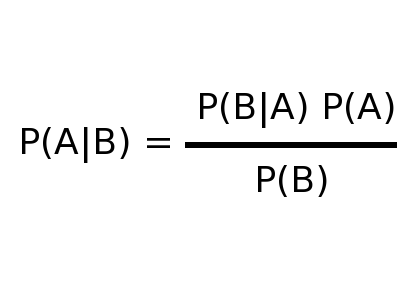
\includegraphics[height=55truemm]{bayes_rule}
  \caption{Bayes' rule geeft de kans dat een Hypothese A waar is gegeven het bewijs B.}
  \label{fig:bayes_rule}
\end{figure}
Bayes' rule geeft de kans dat een hypothese waar is in een wereld waar er al dan niet bewijs is over deze wereld. PPl's kunnen hetzelfde berekenen aan de hand van een inferentie proces dat de taal implementeert. Elke PPL heeft een methode om de inferentie te bereken. Hoe ze dit doen verschilt voor elke PPL. Meer info over de inferentie methodes in de sectie~\ref{subsec:problog2} en~\ref{subsec:anglican}.
\\\\
Het berekenen van de inferentie is een zeer krachtig, maar zeer kostelijk proces qua rekenkracht. Veel PPL's zoeken een balans tussen hoe efficient ze inferentie kunnen berekenen en welke problemen ze kunnen modelleren (hoe expressief de taal is).
\subsection{ProbLog2}
\label{subsec:problog2}
ProbLog is een speciale vorm van PPL. Het is een Probabilistische logische programma PLP. 
ProbLog is gebasseerd op Prolog. Terwijl het niet echt een extensie is van Prolog heeft het wel dezelfde syntax. Het verschil met Prolog zit hem in de kansen dat voor de feiten of predicaten kunnen gezet worden. In Prolog is een feit altijd waar in het programma. In ProbLog is een feit waar met kans P en niet waar met kans (1-P). hetzelfde geldt voor predicaten. Als we een feit schrijven zonder kans is deze waar in het logische programma. Als we een feit schrijven als P::f dan is de feit f waar met kans P en niet waar met kans (P-1). 

\subsubsection{inferentie}
De inferentie in ProbLog gebeurd aan de hand van verschillende processen:
\begin{enumerate}
	\item converteren van logisch programma gewogen booleaanse formules.
	\item inferentie proces op de gewogen booleaanse formules.
\end{enumerate}
Deze stappen zijn onafhankelijke processen en zijn zo gekozen dat de output van het ene algoritme in het volgende algoritme past.

om te converteren van logisch programma gewogen booleaanse we 3 input's nodig. Het ProbLog model, het bewijs van het model en de vragen die men aan het model wilt stellen. Tijdens dit proces wordt het domein van de probabilistische variabelen opgesteld en deze variabelen zullen enkel de termen in hun domein gebruiken om het gewogen booleaanse formula op te bouwen.
\\\\
De inferentie is anders afhankelijk van wat er gevraagt wordt.
\begin{itemize}
	\item Als de MARG/SUCC gevraagt wordt maakt het systeem gebruik van een algoritme genaamd Weighted Model Counting (WMC).
	\item Als de MPE gevraagt wordt maakt het systeem gebruik van een algoritme genaamd MAX-SAT.
\end{itemize}
Dit zijn welbestudeerde algoritmes en voor meer informatie kunt u het artikel (Inference and Learning in Probabilistic Logic Programs using Weighted Boolean Formulas) lezen.
\subsection{Anglican}
\label{subsec:anglican}
\subsubsection{inferentie}

\subsection{Stappenplan}
Om PPL's te evalueren en vergelijken maak ik gebruik van een case study. Ik gebruik een case study omdat het evalueren van programmeer talen die niet dezelfde programmeer paradigma hebben niet triviaal is. De case die ik gebruik is een zelf verzonnen spel dat probabilistische aspecten bevat. Dit spel modelleer ik in ProbLog en Anglican. Na de implementatie kan ik beginnen met het vergelijken en evalueren van de PPL's aan de hand van verschillende kwalitatieve en kwantitatieve criteria.
\subsubsection{Spel}
Het spel bestaat uit een bord van 10 op 10 blokken. Elke blok in het bord heeft 1 toegewezen kleur. Er zijn 4 kleuren die aan een blok kunnen toegewezen worden: rood, groen, geel, blauw.\\\\
Elke beurt kan de speler op 1 van de blokken drukken. Als er op een blok wordt gedrukt, verandert deze van kleur. De kleur waar de blok in verandert hangt af van welke kleur de blok had voor dat er op gedrukt werd.
\begin{itemize}
  \item Een rode blok verandert met 1/3 kans in een groene blok, 1/3 kans in een blauwe blok en 1/3 kans in een gele blok.
  \item Een groene blok verandert met 1/3 kans in een rode blok, 1/3 kans in een blauwe blok en 1/3 kans in een gele blok.
  \item Een blauwe blok verandert met 1/3 kans in een rode blok, 1/3 kans in een groene blok en 1/3 kans in een gele blok.
  \item Een gele blok verandert met 1/3 kans in een rode blok, 1/3 kans in een groene blok en 1/3 kans in een blauwe blok.
\end{itemize}
\begin{figure}
  \centering
    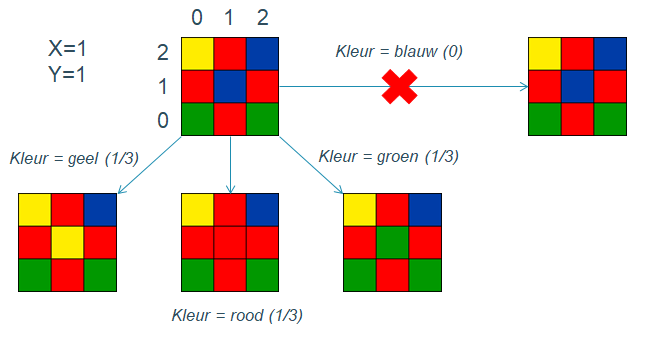
\includegraphics[height=55truemm]{game_change_blocks}
  \caption{In de figuur gebruik ik een 3x3 bord, als er op de middelste blauwe blok (1,1) wordt gedrukt, verandert de blok met 1/3 kans in een rode blok, met 1/3 kans in een groene en met 1/3 kans in een gele blok. De blauwe blok zal nooit in een blauwe blok veranderen. }
  \label{fig:game_change_blocks}
\end{figure}
Figuur~\ref{fig:game_change_blocks} geeft een visuele weergave van wat er gebeurd als er op een blok wordt gedrukt.\\\\
Als er drie of meer blokken van dezelfde kleur horizontaal/verticaal naast elkaar liggen verdwijnen ze en dit levert punten op. De blokken die zich boven de verdwenen blokken bevinden vallen naar beneden tot ze op een andere blok belanden ofwel op de bodem van het spelbord. De bedoeling van het spel is om in tien beurten zoveel mogelijk punten te behalen waarin de speler in elke beurt \'{e}\'{e}n blok van kleur kan veranderen. De beurt eindigt wanneer er geen 3 blokken van dezelfde kleur meer horizontaal en/of verticaal naast elkaar staan.
\begin{figure}
  \centering
    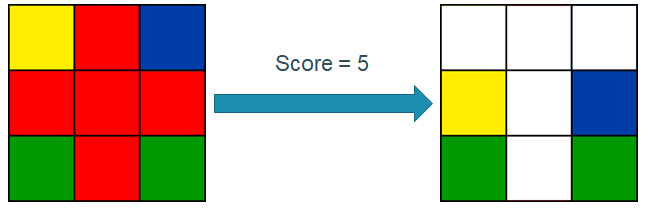
\includegraphics[height=18truemm]{game_score}
  \caption{Stel dat de blok in figuur~\ref{fig:game_change_blocks} rood werd, dan staan er 3 blokken met dezelfde kleur naast elkaar. Het spel verwijdert deze blokken en voor elke blok die verwijdert is krijgt de speler een punt. In dit geval heeft de speler 5 punten. De gele en de blauwe blok vallen naar beneden tot ze op een andere blok of op de bodem vallen.}
  \label{fig:game_score}
\end{figure}
\subsubsection{Modelleren}
\subsubsection{Evaluatiecriteria}
De evaluatiecriteria kunnen gecategorizeerd worden in qualitatieve en quantitatieve criteria. Ook zijn er objectieve criteria en subjectieve criteria waar ik mijn evaluatie op basseer.

\chapter{Resultaten}
\chapter{Conclusie}


\newpage
% ----------------------- Achterblad ------------------------------
% Vergeet niet de tekst aan te passen:
% - Afdeling
% - Adres van de afdeling
% - Telefoon en faxnummer
% -----------------------------------------------------------------
\thispagestyle{empty}
\sffamily
%
\begin{textblock}{191}(113,-11)
{\color{blueline}\rule{160pt}{5.5pt}}
\end{textblock}
%
\begin{textblock}{191}(168,-11)
{\color{blueline}\rule{5.5pt}{59pt}}
\end{textblock}
%
\begin{textblock}{183}(-24,-11)
\textblockcolour{}
\flushright
\fontsize{7}{7.5}\selectfont
\textbf{Faculteit Computerwetenschappen}\\
Geel Huis, Kasteelpark Arenberg 11 bus 2100\\
3001 LEUVEN, BELGI\"{E}\\
tel. + 32 16 32 14 01\\
%fax + 32 16 00 00 00\\
www.kuleuven.be\\
\end{textblock}
%
\begin{textblock}{191}(154,-7)
\textblockcolour{}
\includegraphics*[height=16.5truemm]{sedes}
\end{textblock}
%
\begin{textblock}{191}(-20,235)
{\color{bluetitle}\rule{544pt}{55pt}}
\end{textblock}
\end{document}
